        \documentclass{article}
\usepackage[margin=1in]{geometry}
\usepackage{hyperref}
\usepackage{amsmath,amsfonts,amssymb,amsthm,commath,dsfont}
\usepackage{enumitem}
\usepackage{framed}
\usepackage{xspace}
\usepackage{booktabs}
\usepackage{microtype}
\usepackage{float}
\usepackage[round]{natbib}
\usepackage{cleveref}
\usepackage[dvipsnames]{xcolor}
\usepackage{graphicx}
\usepackage{listings}
\usepackage[breakable]{tcolorbox}
\tcbset{breakable}
\usepackage{mathtools}
\usepackage{subcaption}
%\usepackage{symbols}


\usepackage{pifont}
\newcommand{\cmark}{\ding{51}}
\newcommand{\xmark}{\ding{55}}

\newcommand{\colbar}{\rule[-3mm]{.3mm}{1.5em}}
\newcommand{\rowbar}{\rule[.5ex]{1.5em}{.3mm}}
\DeclareMathOperator{\rank}{rank}

% following loops stolen from djhsu
\def\ddefloop#1{\ifx\ddefloop#1\else\ddef{#1}\expandafter\ddefloop\fi}
% \bbA, \bbB, ...
\def\ddef#1{\expandafter\def\csname bb#1\endcsname{\ensuremath{\mathbb{#1}}}}
\ddefloop ABCDEFGHIJKLMNOPQRSTUVWXYZ\ddefloop

% \cA, \cB, ...
\def\ddef#1{\expandafter\def\csname c#1\endcsname{\ensuremath{\mathcal{#1}}}}
\ddefloop ABCDEFGHIJKLMNOPQRSTUVWXYZ\ddefloop

% \vA, \vB, ..., \va, \vb, ...
\def\ddef#1{\expandafter\def\csname v#1\endcsname{\ensuremath{\boldsymbol{#1}}}}
\ddefloop ABCDEFGHIJKLMNOPQRSTUVWXYZabcdefghijklmnopqrstuvwxyz\ddefloop

% \valpha, \vbeta, ...,  \vGamma, \vDelta, ...,
\def\ddef#1{\expandafter\def\csname v#1\endcsname{\ensuremath{\boldsymbol{\csname #1\endcsname}}}}
\ddefloop {alpha}{beta}{gamma}{delta}{epsilon}{varepsilon}{zeta}{eta}{theta}{vartheta}{iota}{kappa}{lambda}{mu}{nu}{xi}{pi}{varpi}{rho}{varrho}{sigma}{varsigma}{tau}{upsilon}{phi}{varphi}{chi}{psi}{omega}{Gamma}{Delta}{Theta}{Lambda}{Xi}{Pi}{Sigma}{varSigma}{Upsilon}{Phi}{Psi}{Omega}{ell}\ddefloop

\newcommand\T{{\scriptscriptstyle\mathsf{T}}}
\def\diag{\textup{diag}}



\def\SPAN{\textup{span}}
\def\tu{\textup{u}}
\def\R{\mathbb{R}}
\def\E{\mathbb{E}}
\def\Z{\mathbb{Z}}
\def\be{\mathbf{e}}
\def\nf{\nabla f}
\def\veps{\varepsilon}
\def\cl{\textup{cl}}
\def\inte{\textup{int}}
\def\dom{\textup{dom}}
\def\Rad{\textup{Rad}}
\def\lsq{\ell_{\textup{sq}}}
\def\hcR{\widehat{\cR}}
\def\hcRl{\hcR_\ell}
\def\cRl{\cR_\ell}
\def\hcE{\widehat{\cE}}
\def\cEl{\cE_\ell}
\def\hcEl{\hcE_\ell}
\def\eps{\epsilon}
\def\1{\mathds{1}}
\newcommand{\red}[1]{{\color{red} #1}}
\newcommand{\blue}[1]{{\color{blue} #1}}
\def\srelu{\sigma_{\textup{r}}}
\def\vsrelu{\vec{\sigma_{\textup{r}}}}
\def\vol{\textup{vol}}

\newcommand{\ip}[2]{\left\langle #1, #2 \right \rangle}
\newcommand{\mjt}[1]{{\color{blue}\emph\textbf{[M:}~#1~\textbf{]}}}
\newcommand{\sahand}[1]{{\color{green}\emph\textbf{[Sah:}~#1~\textbf{]}}}

\newtheorem{fact}{Fact}
\newtheorem{lemma}{Lemma}
\newtheorem{condition}{Condition}
\theoremstyle{definition}
\theoremstyle{remark}
\newtheorem{remark}{Remark}
\newtheorem{example}{Example}

\newenvironment{Q}
{%
	\clearpage
	\item
}
{%
	\phantom{s} %lol doesn't work
	\bigskip
	\textbf{Solution.}
}

\title{CS 446 / ECE 449 --- Homework 3}
\author{\emph{acard6}}
\date{Version 1.1}

\begin{document}
	\maketitle
	
	\noindent\textbf{Instructions.}
	\begin{itemize}
		\item
		Homework is due \textbf{\color{red}Tuesday, March 02, at noon CDT}.
		
		\item
		Everyone must submit individually at gradescope under \texttt{hw3} and \texttt{hw3code}.
		
		\item
		The ``written'' submission at \texttt{hw3} \textbf{must be typed}, and submitted in
		any format gradescope accepts (to be safe, submit a PDF).  You may use \LaTeX, markdown,
		google docs, MS word, whatever you like; but it must be typed!
		
		\item
		When submitting at \texttt{hw3}, gradescope will ask you to mark out boxes
		around each of your answers; please do this precisely!
		
		\item
		Please make sure your NetID is clear and large on the first page of the homework.
		
		\item
		Your solution \textbf{must} be written in your own words.
		Please see the course webpage for full academic integrity information.
		Briefly, you may have high-level discussions with at most 3 classmates,
		whose NetIDs you should place on the first page of your solutions,
		and you should cite any external reference you use; despite all this,
		your solution must be written in your own words.
		
		\item
		We reserve the right to reduce the auto-graded score for
		\texttt{hw3code} if we detect funny business (e.g., your solution
		lacks any algorithm and hard-codes answers you obtained from
		someone else, or simply via trial-and-error with the autograder).
		
		\item
		When submitting to \texttt{hw3code}, only upload \texttt{hw3\_vae.py} and \texttt{hw3\_gan.py}. Additional files will be ignored.
		
	\end{itemize}
	
	\noindent\textbf{Version History.}
	\begin{enumerate}[leftmargin=3\parindent]
		\item[1.0]
		Initial Version.
		\item[1.1]
		Update code/hw3\_vae.py.
	\end{enumerate}
	
	
	\begin{enumerate}[font={\Large\bfseries}]
		\begin{Q}
	\textbf{\Large Variational Auto-Encoders [Written]}\\
	We use VAEs to learn the distribution of the data $x$. Let $z$ denote the
	unobserved latent variable. We refer to the approximated posterior $q_\phi(z|x)$ as the encoder
	and to the conditional distribution $p_\theta(x|z)$ as the decoder. Use these names to answer
	the following questions.
	\begin{enumerate}
		\item We are interested in modeling data $x \in \{0,1\}^{G}$. Hence, we choose $p_\theta(x|z)$ to follow $G$ independent Bernoulli distributions. Recall, a Bernoulli distribution has a probability density function of 
		$$
		P(k)= 
		\begin{cases}
		1-p & \text{if } k = 0\\
		p    & \text{if } k = 1
		\end{cases}.
		$$
		Use $\hat{y}_j$ to denote the $j^\text{th}\in[1,G]$ dimension of the decoder's output, and similarly $x_j$ the $j^\text{th}\in[1,G]$ dimension of the data $x$. Write down the explicit form for $p_\theta(x|z)$ in terms of $\hat{y}_j$ and $x_j$. 
		
		\item We further assume that $z \in \mathbb{R}^{2}$ and that $q_\phi(z|x)$ follows a multi-variate Gaussian distribution with an identity covariance matrix. What is the output dimension of the encoder?
		
		\item  We want to maximize the log-likelihood $\log p_\theta(x)$. To this end we introduce a joint distribution $p_\theta(x,z)$ and reformulate the log-likelihood via
		$$
		\log p_\theta(x) = \log \sum_z q_{\phi}(z|x) \frac{p_\theta(x,z)}{q_{\phi}(z|x)}.
		$$
		Use Jensen's inequality to obtain a bound on the log-likelihood and divide the bound into two parts, one of which is the Kullback-Leibler divergence $\text{KL}(q_{\phi}(z|x), p(z)).$
		
		\item State at least two properties of the KL-divergence.
		
		
		\item Recall, the evidence lower bound (ELBO) of the log likelihood, $\log p_{\theta}(x)$, is 
		\begin{equation}\label{eq:elbo1}
		\mathbb{E}_{q_\phi(z|x)} [\log p_\theta(x|z)] - \text{KL}(q_\phi(z|x), p(z)).
		\end{equation}
		We can also write the ELBO as
		\begin{equation}
		\mathbb{E}_{q_\phi(z|x)} [\log p_\theta(x|z) + \log p(z) - \log(q_\phi(z|x)].
		\label{eq:elbo2}
		\end{equation}
		{\bf Practically}, will training a VAE using the formulation in Eq. \ref{eq:elbo1} be the same as the one in Eq. \ref{eq:elbo2}? If not, why use one formulation over another?
		\item Observe that the ELBO in Eq.~\ref{eq:elbo1} works for any $q_\phi$ distribution. Is it a good idea to choose $q_\phi(z|x) := \cN(0, I)$? In other words, why is an encoder necessary?
		
		
		\item Let
		$$
		q_{\phi}(z|x) = \frac{1}{\sqrt{2\pi\sigma_{\phi}^2}} \exp\left(-\frac{1}{2\sigma_{\phi}^2}(z - \mu_{\phi})^2\right).
		$$
		What is the value for the KL-divergence $\text{KL}(q_{\phi}(z|x), q_{\phi}(z|x))$ and why?
		\item Further, let
		$$
		p(z) =  \frac{1}{\sqrt{2\pi\sigma_{p}^2}} \exp\left(-\frac{1}{2\sigma_{p}^{2}}(z - \mu_p)^2\right).
		$$
		Note the difference of the means for $p(z)$ and $q_{\phi}(z|x)$ while their standard deviations are identical. Assume that $\sigma=\sigma_{\phi}=\sigma_{p}$. What is the value for the KL-divergence $\text{KL}(q_{\phi}(z|x), p(z))$ in terms of $\mu_p$, $\mu_{\phi}$ and $\sigma$?
		
		\item Now, let $q_{\phi}(z|x)$ and $p(z)$ be  arbitrary probability distributions. We want to find that $q_{\phi}(z|x)$ which maximizes 
		$$
		\sum_z q_{\phi}(z|x)\log p_\theta(x|z) - \text{KL}(q_{\phi}(z|x), p(z))	
		$$
		subject to $\sum_z q_{\phi}(z|x) = 1$. Ignore the non-negativity constraints. State the Lagrangian and compute its stationary point, i.e., solve for $q_{\phi}(z|x)$ which depends on $p_\theta(x|z)$ and $p(z)$. Make sure to get rid of the Lagrange multiplier.
		\item Which of the following terms should $q_{\phi}(z|x)$ be equal to: 
		(1) $p(z)$; (2) $p_\theta(x|z)$; (3) $p_\theta(z|x)$; (4) $p_\theta(x, z)$.
	\end{enumerate}
\end{Q}


        
		%\input{vae_sol.tex}   
		\begin{itemize}
			\item[\textit{Answer A.)}] we know that the $p_{\theta}(x|z) = \prod_{j} p(x_j | z)$, knwoing that $p(x_j=1) = \hat{y}_j \text{ and } p(x_j=0) = 1-\hat{y}_j$ we can 
			formulate $p_{\theta}(x|z) = \prod_{j=1}^{G} (\hat{y}_{j})^{x_{j}} (1-\hat{y}_{j})^{1-x_{j}}$

			\item[\textit{Answer B.)}] if $z \in \mathbb{R}^2$ and $q_{\Phi}(z|x) = \mathcal{N}(\mu, \sigma^2I)$, and if I is 2d the the encoder is also 2d since the 
			identity matrix has to match up with the latent variable.

			\item[\textit{Answer C.)}] By reformulating the log-likelihood to $\log p_{\theta}(x) = \log \sum_z q_{\Phi}(z|x) \frac{p_{\theta}(x,z)}{p_{\theta}(z|x)}$\\
			we can then write it as $\log \sum_z q_{\Phi}(z|x) \frac{p_{\theta}(x,z)}{q_{\Phi}(z|x)} \frac{q_{\Phi}(z|x)}{p_{\theta}(z|x)}$\\ (since we can approximate
			$p_{\theta}(z|x) \approx q_{\Phi}(z|x)$) we then use jensen ineq on the log to get\\
			$\log \sum_z q_{\Phi}(z|x) \frac{p_{\theta}(x,z)}{q_{\Phi}(z|x)} \frac{q_{\Phi}(z|x)}{p_{\theta}(z|x)}$ 
			$\leq \sum_z q_{\Phi}(z|x) \log (\frac{p_{\theta}(x,z)}{q_{\Phi}(z|x)} \frac{q_{\Phi}(z|x)}{p_{\theta}(z|x)})$\\
			$= \sum_z q_{\Phi}(z|x) \log \frac{p_{\theta}(x,z)}{q_{\Phi}(z|x)} + \sum_z q_{\Phi}(z|x) \log \frac{q_{\Phi}(z|x)}{p_{\theta}(z|x)}$
			$= \mathcal{L}(p_{\theta}, q_{\Phi}) + KL(q_{\Phi}, p_{\theta})$ so\\ 
			$\mathcal{L}(p_{\theta}, q_{\Phi}) + KL(q_{\Phi}, p_{\theta} \geq \mathcal{L}(p_{\theta}, q_{\Phi})$

			\item[\textit{Answer D.)}] Properties of KL divergence include, relative entropy is always non-negative, no upper bound exist for the general case,
			and relative entropy remains well-defined for continuous distributions, and furthermore is invariant under parameter transformations.

			\item[\textit{Answer E.)}] yes they are the same since we can rewrite the expectation as\\
			$\mathbb{E}_{q_{\Phi}(z|x)}[\log p(x|z) + \log p(z) - \log q(z|x)]$
			$ = \mathbb{E}_{q_{\Phi}(z|x)}[\log p(x|z)] + \mathbb{E}_{q_{\Phi}(z|x)}[\log p(z) - \log q(z|x)]$ 
			using the subtraction properties of 2 logs we can then combine them and expand the definition of expectation to become\\
			$\mathbb{E}_{q_{\Phi}(z|x)}[\log p(x|z)] + \mathbb{E}_{q_{\Phi}(z|x)}[\log \frac{p(z)}{q(z|x)}]$ 
			$ = \mathbb{E}_{q_{\Phi}(z|x)}[\log p(x|z)] + \sum_z q_{\Phi}(z|x) \log \frac{p(z)}{q_{\Phi}(z|x)}$ we can then substitute with 
			the definition of KL divergence of $-KL(q_{\Phi}, p) = \int_z q_{\Phi}(z|x) \log \frac{p(z)}{q_{\Phi}(z|x)}$.
			By substituting we can reach the conclusion that eq. 1 and eq. 2 are infact the same

			\item[\textit{Answer F.)}] if we use the identity matrix for the prior we assume that each sample of q is i.i.d with a normal distribution,
			which may not perfectly reflect the reality of the nature of real world data. An encoder is necessary to map out helps us extract the most 
			from an image in the form of data and establish useful correlations between various inputs within the network.
			
			\item[\textit{Answer G.)}] KL-divergence is defined part E can be further simplified as\\
			$-KL(q_{\Phi}, p) = \int_z q_{\Phi}(z|x) \log \frac{p(z)}{q_{\Phi}(z|x)} = -\int q \log q + \int q \log p$\\
			if p=q and q is a gaussian distribution then we get that\\ 
			$\int_z q \log q dz= \int_z \frac{1}{\sqrt{2\pi \sigma_q^2}} \exp{(-\frac{(z-\mu_q)^2}{2\sigma^2_q})}*(-\frac{1}{2}\log(2\pi\sigma_q^2))*(-\frac{(z-\mu_q)^2}{2\sigma^2_q})dz$
			$ = -\frac{1}{2}(1+ \log 2\pi\sigma_q^2)$, \\
			doing the same for KL(q,p) we get\\
			$-\int_z q \log p dz =\\ -\int_z \frac{1}{\sqrt{2\pi \sigma_p^2}} \exp{(-\frac{(z-\mu_p)^2}{2\sigma^2_p})}*(-\frac{1}{2}\log(2\pi\sigma_p^2))*(-\frac{(z-\mu_p)^2}{2\sigma^2_p}) dz$
			$ = \frac{1}{2} \log 2\pi\sigma_p^2 + \frac{\sigma_q^2 + (\mu_q - \mu_p)^2}{2\sigma_p^2}$\\
			combining the 2 parts we can simplify and get\\ 
			$KL(q,p) = log \frac{\sigma_2}{\sigma_1}+ \frac{\sigma_1^2+(\mu_1-\mu_2)^2}{2\sigma_2^2} - \frac{1}{2}$
			sice they're eqaul log(1)=0, the means cancel, and the ratio of the variance is 1 which resolves to 1/2 
			
			\item[\textit{Answer H.)}] using the equation of KL from the last part of\\
			$KL(q,p) = log \frac{\sigma_p}{\sigma_{\Phi}}+ \frac{\sigma_{\Phi}^2+(\mu_{\Phi}-\mu_p)^2}{2\sigma_p^2} - \frac{1}{2}$\\
			since the variance/std is the same between p and q their ratio is just 1 leaving the equation to be equal to\\
			$K(q,p) = log \frac{\sigma}{\sigma}+ \frac{\sigma^2+(\mu_{\Phi}-\mu_p)^2}{2\sigma^2} - \frac{1}{2}$
			$ = \frac{\sigma^2+(\mu_{\Phi}-\mu_p)^2}{2\sigma^2} - \frac{1}{2}$
			
			\item[\textit{Answer I.)}] $L(q_{\Phi},\lambda) = \sum_z q_{\Phi} \log p_{\theta} - KL(q_{\Phi}, p(z)) + \lambda((\sum_z q_{\Phi}(z|x)) -1)$\\
			$\frac{\delta L}{\delta q_{\Phi}} = \log p_{\theta} - \log q_{\Phi} - 1 - \lambda = 0 \rightarrow$
			$\log q_{\Phi} = \log p_{\theta} - \lambda - 1 \rightarrow$\\
			$\sum_z q_{\Phi} = \sum_z \exp (\log p_{\theta}-(\lambda+1)) = 1$ take the log of 1 and q to get\\
			$\log \sum_z \exp (\log p_{\theta}-(\lambda+1))=0 \rightarrow$
			$\frac{\delta}{\delta \lambda} \sum_z \exp (\log  p_{\theta}-(\lambda+1)) = \sum_z \exp (\log  p_{\theta}-\lambda) = 1$\\
			multiply by p(z) on both sides $\sum_z p(z) \exp (\log p_{\theta}-\lambda) = p(x)$, take the log of both sides\\
			$\log p(x) = log \sum_z p(z) \exp ( \log p_{\theta} - \lambda) = \sum_z p(z) \log p_{\theta} - \lambda$
			using jensen ineq we note thet $\log p(x) < \sum_z p(z) \log p_{\theta} - \lambda = $\\
			$p(x) <= \exp \sum_z p(z) \log p_{\theta} - \lambda$ therefore $q(z|x)$ is maximized by 
			$q_{\Phi} = p(z) \exp (\log (p_{\theta}(x|z)))$, when we ger rid of the lagrangian by taking the sum over all q over z is equal to 1


			\item[\textit{Answer J.)}] $q_{\Phi}(z|x)$ should be set equal to $p_{\theta}(z|x)$ since we can closely approximate probability $p(z|x)$ as $q(z|x)$

		\end{itemize}
		
		\begin{Q}
	\textbf{\Large Variational Auto-Encoders [Coding]}\\
	
	In this assignment, you will implement a Variational Autoencoder and train it on  MNIST
	digits. Each datapoint $x$ in the MNIST dataset is a $28 \times 28$ grayscale image (i.e., pixel values are between 0 and 1) of a handwritten digit in $\{0, \dots, 9\}$, and a label indicating which number. The prior over each digit's latent representation $z$ is a multivariate standard normal distribution, i.e., $z \sim \mathcal{N}(0,I) $. For all questions, we set the dimension of the latent space $D_z$ to 2. Given the latent representation $z$ for an image, the distribution over all $784$ pixels in the image is given by a product of independent Bernoulli, whose characteristic probabilities are given by the output of a neural network $f_{\theta}(z)$ (the decoder):
	\begin{equation}
	p_{\theta}(x|z) = \prod_{d=1}^{784} \text{Ber}(x_{d}|f_{\theta}(z) ).
	\end{equation}
	\textbf{Relevant files: } \textit{hw3\_vae.py}, \textit{hw3\_utils.py}.
	
	\begin{enumerate}
		\item  \textbf{Decoder Architecture}.
		Given a latent representation $z$, the decoder produces a $784$-dimensional vector representing the Bernoulli distribution characteristic probability, i.e., the probability for every pixel in the image being labeled 1. Define the decoder parameters in the method \textit{\_\_init\_\_}  of the \textit{Decoder} class and implement the corresponding \textit{forward} function. The decoder architecture is a multi-layer perceptron (i.e., a fully-connected neural network), with two hidden layers, followed each by a non linearity: \textit{tanh} after the first layer and \textit{sigmoid} after the second layer. The hidden dimension is set to 500 units.
		
		\item \textbf{Distributions}.
		\begin{enumerate}
			\item Implement the method \textit{logpdf\_diagonal\_gaussian} that, given a latent representation $z$, a mean $\mu$ and the variance $\sigma^2$, outputs the log-likelihood of the normal distribution  $\mathcal{N}(\mu,\sigma^2 I)$.
			
			\item  Implement a function \textit{logpdf\_bernoulli} that, given a sample $x$ and a probability $p$,  outputs the log-likelihood of a Bernoulli distribution.
			
			\item  Implement the function \textit{sample\_diagonal\_gaussian} which uses the reparametrization trick to sample $z$ from Diagonal Gaussian $z \sim \mathcal{N}(\mu,\sigma^2 I)$.
			\item  Implement the function \textit{sample\_Bernoulli} which samples a configuration $x$ from a Bernoulli distribution characterized by a probability $p$.
		\end{enumerate}
		
		\item  \textbf{Variational Objective}. Complete the function \textit{elbo} with the ELBO loss implementation corresponding to Eq.~\ref{eq:elbo2}. 
		
		
		\item  \textbf{Training}. Train the model for 200 epochs. \textbf{Hint: } Run the \textit{main} function and make sure the number of epochs is set-up correctly in \textit{parse\_args}.
		%or run the following command: \begin{lstlisting}[language=bash] HW5_vae.py --num_epoches 200 \end{lstlisting}
		
		\item \textbf{Visualization}.  
		\begin{enumerate}
			\item \textbf{Samples from the generative model}. Complete the method \textit{visualize\_data\_space} following the instructions:
			
			\begin{itemize}
				\item Sample a $z$ from the prior $p(z)$. Use \textit{sample\_diagonal\_gaussian}.
				\item Use the generative model to parameterize a Bernoulli distribution over $x$ given $z$. Use \textit{self.decoder} and \textit{array\_to\_image}. Plot this distribution $p(x|z)$.
				\item Sample $x$ from the distribution $p(x|z)$. Plot this sample.
				\item Repeat the steps above for 10 samples $z$ from the prior. Concatenate all your plots into one $10\times2$ figure where the first column is the distribution over $x$ and the second column is a sample from this distribution. Each row will be a new sample from the prior. Hint: use the function \textit{concat\_images}.
				\item Attach the figure to your report.
			\end{itemize}
			\item \textbf{Latent space visualization}. Produce a scatter plot in the latent space, where each point in the plot represents a different image in the training set. Complete the method \textit{visualize\_latent\_space} following the instructions:
			\begin{itemize}
				\item  Encode each image in the training set. Use \textit{self.encoder}.
				\item Plot the mean vector $\mu$ of $q_{\phi}(z|x)$ in the 2D latent space with a scatter plot. Make sure to color each point according to the class label (0 to 9). 
				\item Attach the scatter plot to your report.
			\end{itemize}
			\item  \textbf{Interpolation between two classes}. Complete the method \textit{visualize\_inter\_class\_interpolation} following the instructions:
			\begin{itemize}
				\item  Sample 3 pairs of data points (\textit{self.train\_images}) with different classes (\textit{self.train\_labels}).
				\item  Encode the data in each pair, and take the mean vectors. Note that the encoder produces a mean vector and a variance one.
				\item  Interpolate between these mean vectors. We denote the output by $z_{\alpha}$, with $\alpha \in [0,1]$ and the interpolation step being 0.1. Hint:  use the function \textit{interpolate\_mu}.
				\item Along the interpolation, plot the distributions $p(x|z_{\alpha})$ in the same figure.
				\item Use \textit{concat\_images} to concatenate these plots into one figure.
				\item Attach the plot to your report.
			\end{itemize}
		\end{enumerate}
		
	\end{enumerate}
	
	
\end{Q}


        
		%\input{vae_coding_sol.tex}
		\begin{center}
			
			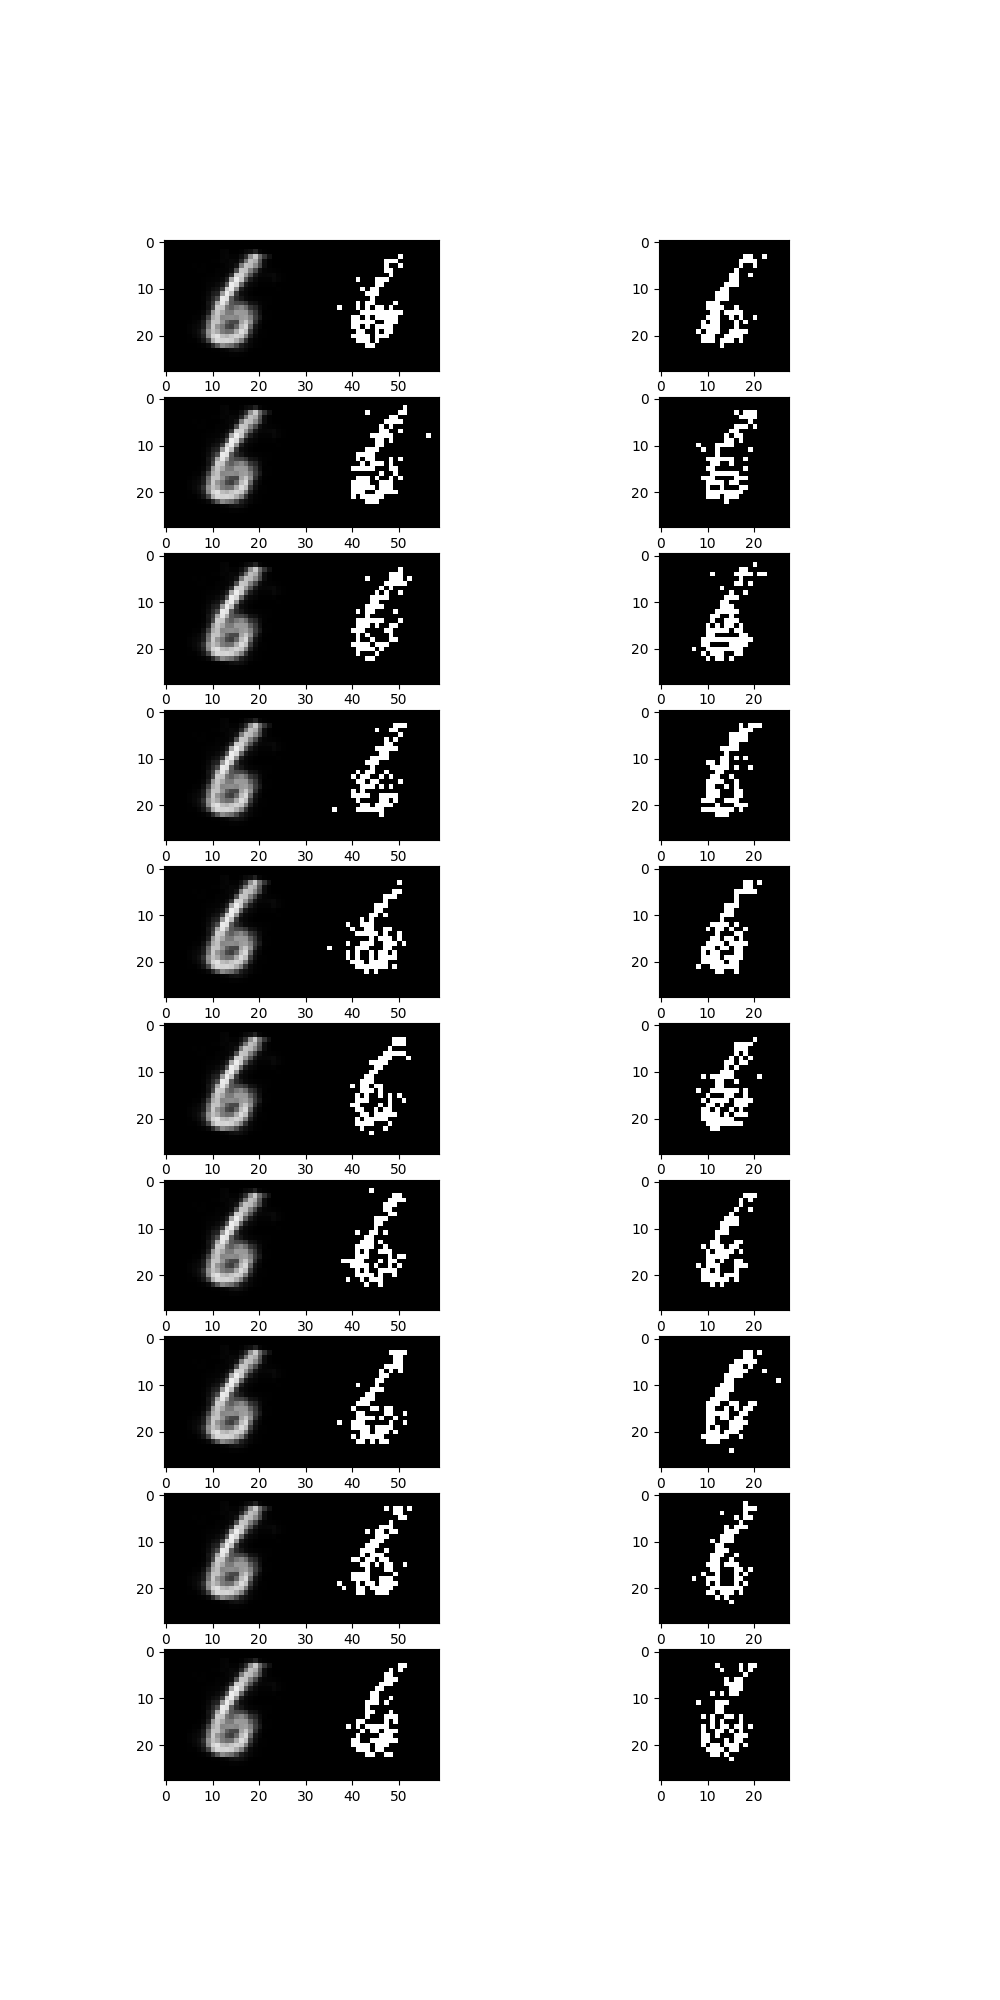
\includegraphics[scale=0.5]{data_space.png}\\
			\textbf{figure 1:} epoch = 0\\


		\end{center}


		\begin{Q}
\textbf{\Large Generative Adversarial Networks [Written]}\\

Here we discuss distribution-comparison-related problems in Generative Adversarial Networks (GANs).

\begin{enumerate}
	\item What is the cost function for classical GANs? Use $D_{\omega} (x)$ as the discriminator and $G_\theta(x)$ as the generator.
	
	\item Assume arbitrary capacity for both discriminator and generator. In this case we refer to the discriminator using $D(x)$, and denote the distribution on the data domain induced by the generator via $p_G (x)$. State an equivalent problem to the one asked for in part (a), by using $p_G (x)$.
	
	\item Assuming arbitrary capacity, derive the optimal discriminator $D^\ast(x)$ in terms of $p_\text{data}(x)$ and $p_G(x)$.
	
	\textbf{Hint:} you can think of fixing generator $G(\cdot)$ to find the optimal value for discriminator $D(\cdot)$.
	
% 	\begin{comment}
	
% 	\textbf{Hint:} you may need the Euler-Lagrange equation:
% 	\begin{align*}
% 		\frac{\partial L(x, D, \dot{D})}{\partial D} - \frac{d}{dx} \frac{\partial L(x, D, \dot{D})}{\partial \dot{D}} = 0
% 	\end{align*}
% 	where $\dot{D} = \frac{\partial D}{\partial x}$.
	
% 	\end{comment}
	
	\item Assume arbitrary capacity and an optimal discriminator $D^\ast(x)$ from (c), show that the optimal generator $G^\ast(x)$ generates the distribution $p^\ast_G = p_\text{data}$, where $p_\text{data}(x)$ is the data distribution.
	
	\textbf{Hint:} you may need the Jensen-Shannon divergence:
	\begin{align*}
		\text{JSD}(p_\text{data}, p_G) = \frac{1}{2} \text{KL}(p_\text{data}, M) + \frac{1}{2} \text{KL}(p_G, M),
	\end{align*}
	where $M = \frac{1}{2} (p_\text{data} + p_G)$.
	
	\item More recently, researchers have proposed to use the Wasserstein distance instead of divergences to train the models since the KL divergence often fails to give meaningful information for training. Consider three distributions, $\mathbb{P}_1 \sim U[0, 1]$, $\mathbb{P}_2 \sim U[0.5, 1.5]$, and $\mathbb{P}_3 \sim U[1, 2]$, where $U[a, b]$ is uniform distribution over $[a, b]$. Calculate $\text{KL}(\mathbb{P}_1, \mathbb{P}_2)$, $\text{KL}(\mathbb{P}_1, \mathbb{P}_3)$, $\mathbb{W}_1 (\mathbb{P}_1, \mathbb{P}_2)$, and $\mathbb{W}(\mathbb{P}_1, \mathbb{P}_3)$, where $\mathbb{W}_1(\cdot, \cdot)$ is the Wasserstein-1 distance between two distributions.
	 
	\textbf{Hint:} this subproblem requires no \textit{real} mathematical computation. What you need to do is to understand the intuitive meaning of KL-divergence and Wasserstein distance. You may find wiki of \textit{Earth mover's distance} and \textit{Wasserstein metric} useful.
\end{enumerate}

\end{Q}
          

                    
		%\input{gan_sol.tex}  
		\begin{itemize}
			\item[\textit{Answer A.)}] the classical cost function for a GAN includes the generators cost function and the discriminators loss.
			loss of the discriminator is $loss_d = -\sum_x \log(D_{\omega}(x)) - \sum_z \log(1 - D_{\omega}(G_{\theta}(z)))$. Where as the loss for the generator
			is $loss_g = -\sum_z \log(D_{\omega}(G_{\theta}(z)))$. So the cost is just $cost = loss_d + loss_g$

			\item[\textit{Answer B.)}] using $p_G(x)$ as the distribution on the data domain induced by the generator we get the 
			$-\int_{x} p_{data}(x) \log(D_{\omega}(x))dx - \int_{z} p_z(z) \log(1-D_{\omega}(G_{\theta}(x))) dz =$\\
			$-\int_{x} p_{data}(x) \log(D_{\omega}(x)) + p_G(x) \log(1-D_{\omega}(x)) dx = \int_x L(x,D, \dot{D}) dx$

			\item[\textit{Answer C.)}] The optimal value for the discriminator assuming arbitrary capacity and a fixed G() and D() for our loss L, we find that we derive
			our w.r.t D and set it equal to 0 to get
			$\frac{\delta L(x,D,\dot{D})}{\delta D} = -\frac{p_{data}}{D}+\frac{p_G}{1-D} = 0 \rightarrow D^*(x) = \frac{p_{data}(x)}{p_{data}(x) + p_G(x)}$

			\item[\textit{Answer D.)}] To find the optimal generator we begin by substituting $D^*(x)$ for $ D(x)$ in the equation from part B, we see that we get\\
			$-\int_{x} p_{data}(x) \log(D^*(x)) + p_G(x) \log(1-D^*(x)) dx = \\
			-\int_{x} p_{data}(x) \log(\frac{p_{data}(x)}{p_{data}(x) + p_G(x)}) + p_G(x) \log(1-\frac{p_{G}(x)}{p_{data}(x) + p_G(x)}) dx\\
			= -2JSD(p_{data}, p_G) + \log(4) = JSD(p_{data}, p_G) = -KL(p_{data}, M) - KL(p_G, M) + \log(4)$\\
			which gives us the optimal generator is $p_G(x) = p_{data}(x)$

			\item[\textit{Answer E.)}] the probability of a uniform distribution is $\frac{1}{b-a}$ so to find KL we integrate \\
			$KL(\mathbb{P}_1, \mathbb{P}_2) = \int_{x} p_{\mathbb{P}_1}(x) \log(\frac{p_{\mathbb{P}_1}(x)}{p_{\mathbb{P}_2}(x)}) = 
			\int_{0.5}^{1} \frac{1}{1-0} \log(\frac{ \frac{1}{1-0} }{ \frac{1}{1.5-0.5} })dx =
			\int_{0.5}^{1} \log(1)dx = 0$,\\
			given that the probability of $\mathbb(P)_3$ is also 1, when put into the KL divergence it to goes to 0. For the Wasserstein distance we get that\\
			$W(\mathbb{P}_1, \mathbb{P}_2) = min_{p_j(x,x') \in \prod(\mathbb{P}_1, \mathbb{P}_2)} \mathbb{E}[||x-x'||] = 
			\int f(x) dp_{\mathbb{P}_1}  -\int f(x) dp_{\mathbb{P}_2} \rightarrow\\ 
			W(\mathbb{P}_1, \mathbb{P}_2) = (\int_{0}^{1} |F(x) - G(x)| dx)$, where F and G are the cdf's of $\mathbb{P}_1, \mathbb{P}_2$ respectively, and since 
			G = 1/2F on the interval 0 to 1 we set $2*dp_{\mathbb{P}_2} = dp_{\mathbb{P}_1}$ W to be \\
			$\int_{0}^{1} 2 f(x)-\frac{1}{2} dx = \frac{3}{4}$\\
			We repeat the process for $W(\mathbb{P}_3,\mathbb{P}_3)$ and we note that $\mathbb{P}_3$ is out of the interval 0 to 1 so thus we just get that W is
			just $\int_{0}^{1} \frac{1}{1} dx = 1$

		\end{itemize}
		
		\begin{Q}
	\textbf{\Large Generative Adversarial Networks [Coding]}\\
	
	In this problem, you need to implement a Generative Adversarial Network and train it on MNIST digits.
	
	\begin{table}[h]
		\begin{center}
			\caption{\textbf{Discriminator Architecture}}
			\label{GAN: dis}
			\begin{tabular}{ccccccc}
				\toprule
				{\small\textit{Layer No.}}
				& {\small \textit{Layer Type}}
				& {\small \textit{Kernel Size}}
				& {\small \textit{Stride}}
				& {\small \textit{Padding}}
				% & {\small \textit{Input Dim}}
				% & {\small \textit{Output Dim}}
				% & {\small \textit{Input Channels}}
				& {\small \textit{Output Channels}} \\
				\midrule
				1 & conv2d   & 3 & 1 & 1 & 2 \\
				2 & ReLU     & - & - & - & 2 \\
				3 & MaxPool  & 2 & 2 & - & 2 \\
				4 & conv2d   & 3 & 1 & 1 & 4 \\
				5 & ReLU     & - & - & - & 4 \\
				6 & MaxPool  & 2 & 2 & - & 4 \\
				7 & conv2d   & 3 & 1 & 0 & 8 \\
				8 & ReLU     & - & - & - & 8 \\
				9 & Linear   & - & - & - & 1 \\
				% 10 & ReLU    & - & - & - & 16 \\
				% 11 & Linear  & - & - & - & 1 \\
				\bottomrule
			\end{tabular}
		\end{center}
	\end{table}
	
	\begin{table}[h]
		\begin{center}
			\caption{\textbf{Generator Architecture}}
			\label{GAN: gen}
			\begin{tabular}{ccccccc}
				\toprule
				{\small\textit{Layer No.}}
				& {\small \textit{Layer Type}}
				& {\small \textit{Kernel Size}}
				& {\small \textit{Stride}}
				& {\small \textit{Padding}}
				& {\small \textit{Bias}}
				% & {\small \textit{Input Dim}}
				% & {\small \textit{Output Dim}}
				% & {\small \textit{Input Channels}}
				& {\small \textit{Output Channels}} \\
				\midrule
				1 & Linear             & - & - & - & \cmark & 1568 \\
				2 & LeakyReLU(0.2)     & - & - & - & -      & 1568 \\
				3 & Upsample(scale=2)  & - & - & - & \xmark & 32 \\
				4 & conv2d             & 3 & 1 & 1 & \cmark & 16 \\
				5 & LeakyReLU(0.2)     & - & - & - & -      & 16 \\
				6 & Upsample(scale=2)  & - & - & - & \xmark & 16 \\
				7 & conv2d             & 3 & 1 & 1 & \cmark & 8 \\
				8 & LeakyReLU(0.2)     & - & - & - & -      & 8 \\
				9 & conv2d             & 3 & 1 & 1 & \cmark & 1 \\
				10 & sigmoid           & - & - & - & -      & 1 \\
				\bottomrule
			\end{tabular}
		\end{center}
	\end{table}
	
	\begin{enumerate}
		\item Implement a discriminator \texttt{DNet} in \texttt{hw3\_gan.py} using the architecture described in Tab.\ \ref{GAN: dis}. Layers contain bias if corresponding \texttt{torch} function has an option for adding one.
		
		\textbf{Remark 1:} From layer 8 to layer 9, you need to flatten each data entry from a matrix to a vector.
		
		\item Implement a generator \texttt{GNet} in \texttt{hw3\_gan.py} using the architecture described in Tab.\ \ref{GAN: gen}.
		
		\textbf{Remark 2:} From layer 2 to layer 3, you need to reshape each data to size $(32, 7, 7)$ in the format of \textit{CHW}. Note,  $1568 = 32\times7\times7$.
		
		\textbf{Remark 3:} For (a) and (b), please define layers in \texttt{\_\_init\_\_} with \textbf{exactly the same} order as they appear in Tab.~\ref{GAN: dis} and Tab.~\ref{GAN: gen}.
		
		\textbf{Remark 4:} We have listed \textbf{all} layers for discriminator and generator. No need to add any extra components.
		
		\item Implement the weight initialization function \texttt{\_weight\_init} in \texttt{DNet} and \texttt{GNet}: use \texttt{kaiming\_uniform} for weights and 0 for the bias if the layer contains bias.
		
		\textbf{Hint:} to iterate over all layers of an \texttt{nn.Module}, you may find \texttt{self.children()} useful. See \texttt{children()} function explained in  \url{https://pytorch.org/docs/stable/generated/torch.nn.Module.html}.
		
		\item Implement the loss function for the discriminator: \texttt{\_get\_loss\_d} of \texttt{GAN} class in \texttt{hw3\_gan.py}.
		
		\textbf{Hint:} you may find \texttt{torch.nn.BCEWithLogitsLoss} useful.
		
		\item Implement the loss function for the generator: \texttt{\_get\_loss\_g} of \texttt{GAN} class in \texttt{hw3\_gan.py}.
		
		\textbf{Hint:} you may find \texttt{torch.nn.BCEWithLogitsLoss} useful.
		
		\item Attach generated images after training.
		
		\textbf{Remark 5:} the provided code default saves images during training. You can choose three of the saved ones and indicate the corresponding epochs.
		
		\textbf{Remark 6:} with default training settings, you should obtain reasonable generated images after around 30 epochs.
		
	\end{enumerate}
	
\end{Q}


        
		%\input{gan_coding_sol.tex}     
		\begin{center}
			
			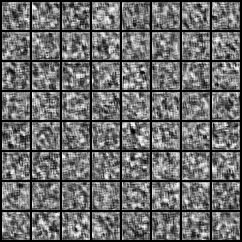
\includegraphics[scale=0.9]{test_0.png}\\
			\textbf{figure 1:} epoch = 0\\

			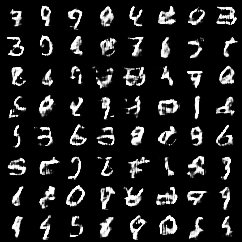
\includegraphics[scale=0.9]{test_30.png}\\
			\textbf{figure 2:} epoch = 30\\

			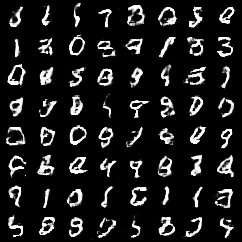
\includegraphics[scale=0.9]{test_70.png}\\
			\textbf{figure 3:} epoch = 70\\

		\end{center}
	\end{enumerate}
\end{document}
